\section{Choosing the documents to read and the resolution a sample reaches}

\subsection{Choosing the documents to read}
\label{sup:design}

A text encoder embeds documents without any human reading and without any call to a large language model. Embedding needs only the documents in hand, so every document a researcher holds can be embedded. On a GPU the cost is small. In this study one GPU embedded the 80{,}634 tweets of the five Census slices with Qwen3 in under 10 minutes. A CPU embeds the same documents more slowly. An encoder offered through a commercial API can be used only when the data may be sent to its provider. Data obtained under a use agreement often may not leave the researcher's machine, so this study used an encoder run locally. A researcher who holds the whole corpus can therefore choose which $n$ documents to read from all of it. We compare random samples of $n$ documents with two designs that choose the $n$ documents from the embedded corpus.

In the first design, the researcher divides the corpus into $n$ groups of similar documents and reads the document nearest the center of each group, the average embedding of the group's documents. $k$-means \citep{lloyd1982} forms the groups by assigning each document to the nearest of $n$ centers and moving each center to the average embedding of its documents, until the groups stop changing. For a sample of 15 documents, $k$-means divides the corpus into 15 groups, and the researcher reads one document from each group. We take this design from work that picks data for a model to learn from \citep{chang2021training,yuan2020coldstart,hacohen2022active,zhang2023autocot}, and we measure how much of the corpus the chosen documents cover.

The second design, greedy maximum coverage, picks the documents one at a time. Each pick is the document that covers the most corpus documents not yet covered, that is, the most documents with no chosen document within $r$. With 15 documents, the first pick is the document with the most other documents within $r$, and each later pick adds the most documents that the earlier picks left uncovered. A set chosen this way covers at least 63\% of what the best possible set of $n$ documents covers \citep{nemhauser1978}. We use the greedy design as a reference for how much a careful choice of $n$ documents can cover. Because the distance from every corpus document to its nearest chosen document is known, we compute the missing mass of a chosen sample exactly, without an estimator.

A researcher who does not hold the whole corpus chooses from the documents that can be obtained. Sometimes a large random sample can be obtained but not the whole corpus, for example because a platform's interface returns only a sample of its posts or because the corpus is too large to store. The researcher then draws a random pool of documents from the corpus and embeds the pool. The researcher chooses the $n$ documents by $k$-means within the pool. The missing mass of the chosen sample is computed from the pool alone, as the percentage of pool documents that were not chosen and have no chosen document within $r$. The chosen documents are left out of this count because each covers itself, the same reason that the factor $1 - n/N$ enters the estimate $G\,(1 - n/N)$. We test pools of 1{,}000 and 5{,}000 documents, five pools of each size, with $n$ of 15 and 100. The tests use nine of the ten real corpora, all but Bluesky, which has no distance that means the same content, at both $r_{\mathrm{same}}$ and $r_{\mathrm{topic}}$. We report what a pool keeps as a share of the gain, the reduction in missing mass that $k$-means on the whole corpus achieves over a random sample of the same size. The share is computed only where this gain exceeds 2 percentage points, because a share of a gain near zero says nothing. Sometimes only the documents to be read can be obtained, for example because each document costs money or requires access. The researcher then draws them at random, embeds them, and estimates their missing mass with $G\,(1 - n/N)$. When the corpus size $N$ is unknown but far larger than $n$, the factor $1 - n/N$ is close to 1, and $G$ alone estimates the missing mass.

\subsection{The resolution a sample reaches}
\label{sup:resolution}

Every random sample covers 80\% of the corpus at some resolution, because a looser resolution $r$ counts more documents as the same content. We call this resolution $r_{80}(n)$, the distance between embeddings within which 80\% of the corpus has a document from a random sample of $n$ documents. We take 80\% as an example of a high level of coverage. We estimate $r_{80}(n)$ from the sample alone as the resolution at which $G\,(1 - n/N)$ equals 20\%, because $G\,(1 - n/N)$ estimates the missing mass. We interpret $r_{80}(n)$ in content through the pairs of documents that the large language models judged at that distance. For those pairs we report the percentage judged the same topic or the same specific content, and the percentage judged the same specific content. When most judged pairs at $r_{80}(n)$ are on the same topic, a corpus document within that distance of a sampled document is usually on the same topic as the sampled document.

\section{Additional results}

\subsection{What a random sample covers}
\label{sup:reader}

Table~\ref{tab:reader} reports the missing mass of random samples from 15 to 1{,}000 documents at two resolutions. At the content level the resolution is $r_{\mathrm{same}}$, so a corpus document counts as covered when the sample contains a document with the same specific content. At the topic level the resolution is $r_{\mathrm{topic}}$, so a sampled document on the same topic is enough. The answer differs between two groups of corpora. The repetitive corpora, the Trump forum and the Census slices selected by a keyword, return again and again to a limited number of claims. The diverse corpora, AskDocs, TIFU, Truth Social and the random Census slice, rarely contain two documents with the same specific content. On the diverse corpora, a random sample covers almost nothing at the content level. Fifteen random documents leave more than 99\% of each diverse corpus with no document of the same specific content in the sample. The largest samples in Table~\ref{tab:reader} still miss between 84\% and 96\% of each diverse corpus. On the repetitive corpora, 15 random posts already show nearly every topic. They leave between 1.8\% and 11\% of each corpus without a post on the same topic. At the content level the same posts miss between 62\% and 98\%. The largest samples still miss between 16\% and 70\% at the content level. The size of a sample alone therefore says little about how much of a corpus it covers.

\begin{figure}[t]
\centering
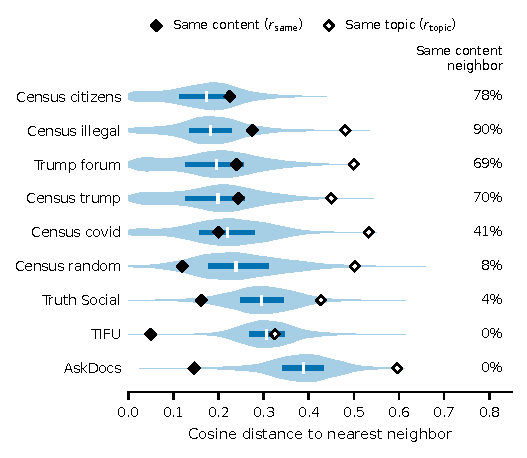
\includegraphics[width=\columnwidth]{figures/spread.pdf}
\caption{In the repetitive corpora, 41\% to 90\% of documents have a nearest neighbor within $r_{\mathrm{same}}$, and in the diverse corpora 8\% or fewer do. Each row is one corpus, with 5{,}000 documents drawn at random, and the rows are ordered by the median distance. The violin shows the cosine distances from each document to its nearest neighbor in the embedding space, with the middle half as a thick bar and the median as a white tick. The filled diamond marks $r_{\mathrm{same}}$ and the open diamond marks $r_{\mathrm{topic}}$. Census citizens has no open diamond, because its percentage of judged pairs on a topic never falls to one half. The number on the right is the percentage of documents whose nearest neighbor lies within $r_{\mathrm{same}}$.}
\label{fig:spread}
\end{figure}

The two groups of corpora differ most in how many of their documents have another document with the same specific content close by. We drew 5{,}000 documents at random from each of the nine corpora and found, for each document, its nearest neighbor, the other document at the smallest cosine distance in the embedding space. We drew the same number from every corpus, because the more documents a corpus contains, the closer each document's nearest neighbor tends to be. A pair closer than $r_{\mathrm{same}}$ is more likely than not to be judged the same content, because the percentage of pairs judged the same content falls as the distance grows and crosses one half at $r_{\mathrm{same}}$. The right-hand column of Figure~\ref{fig:spread} reports, for each corpus, the percentage of documents whose nearest neighbor lies within $r_{\mathrm{same}}$. In the Trump forum and the Census citizens, Census trump and Census illegal slices, this percentage is 69\% to 90\%. In Census covid it is 41\%, because the covid $r_{\mathrm{same}}$ of 0.20 is smaller than the median distance from its documents to their nearest neighbors, 0.22. In the diverse corpora the percentage is 8\% or less, and it is 0\% in AskDocs and TIFU. The median distance to the nearest neighbor, which a reader would look at first, ranges from 0.17 in Census citizens to 0.39 in AskDocs. These medians show the picture one would expect, with tweets on one keyword gathering together and questions and personal stories spreading out. The medians alone mislead, as AskDocs and TIFU show. AskDocs questions lie the farthest apart, yet all but one of them have a nearest neighbor within the AskDocs $r_{\mathrm{topic}}$ of 0.60, which makes a shared topic more likely than not. TIFU stories lie closer together, yet only 62\% of them have a nearest neighbor within the TIFU $r_{\mathrm{topic}}$ of 0.33. The corpus that looks the most spread out is therefore the one where a document most often has a neighbor likely on its topic. The TIFU $r_{\mathrm{same}}$ is only 0.05, because long personal stories differ in their details even when their embeddings are close. For someone who samples, the percentage in the right-hand column is the part of the corpus that is more likely than not to contain a second document with the same content. A document with no second document of the same content can be covered only by reading it, so no choice of documents helps in a corpus where most documents are like that. This explains why $k$-means selection removes almost nothing at the content level on AskDocs, TIFU and Truth Social, and why it covers far more than a random sample on the repetitive corpora (Section~\ref{sup:design-results}). With 15 documents from Census illegal, a random sample misses 63\% of the corpus at the content level, and a $k$-means sample misses 33\%.

\begin{table}[t]
\centering
\small
\setlength{\tabcolsep}{4pt}
\begin{tabular}{lrrrrrr}
\toprule
 & \multicolumn{3}{c}{Same content} & \multicolumn{3}{c}{Same topic} \\
\cmidrule(lr){2-4}\cmidrule(lr){5-7}
Corpus & 15 & 100 & 1{,}000 & 15 & 100 & 1{,}000 \\
\midrule
TIFU & 99.8 & 99.0 & 90.0 & 98.5 & 91.5 & 57.5 \\
AskDocs & 99.8 & 99.0 & 89.9 & 58.3 & 15.4 & 0.7 \\
Truth Social & 99.9 & 99.6 & 96.4 & 63.9 & 32.1 & 10.0 \\
Census random & 99.7 & 98.2 & 84.0 & 15.8 & 7.0 & 2.1 \\
Census covid & 98.0 & 91.6 & 70.2 & 2.3 & 0.4 & 0.0 \\
Census citizens & 89.9 & 67.8 & 33.1 & & & \\
Trump (forum) & 88.0 & 68.0 & 40.2 & 3.6 & 1.0 & 0.1 \\
Census trump & 86.9 & 66.7 & 42.1 & 10.8 & 4.3 & 0.9 \\
Census illegal & 62.5 & 35.1 & 15.9 & 1.8 & 0.6 & 0.2 \\
\bottomrule
\end{tabular}
\caption{The percentage of the corpus that has nothing like it in a random sample of 15, 100 or 1{,}000 documents, at the distance where half of the judged pairs are the same content ($r_{\mathrm{same}}$) or at least the same topic ($r_{\mathrm{topic}}$), both judged by Qwen3.8. True values computed against the whole corpus, averaged over 20 samples. The Census citizens slice has no topic distance, because nearly every pair in it shares the topic.}
\label{tab:reader}
\end{table}

Two cases show the range. A random sample of 15 tweets from the Census illegal slice contains a tweet on the same topic for 98\% of the slice. Only 38\% of the slice has a tweet in the sample that makes the same specific claim. TIFU lies at the other end. Fifteen random stories contain a story on the same topic for only 1.5\% of the corpus. Even 1{,}000 stories contain a story about the same event for only 10\% of the corpus. A reader of 15 tweets from the illegal slice has met nearly every topic of the slice, whereas a reader of 15 TIFU stories has met few of its topics.

A researcher learns which case applies from the sample itself. The estimate $G\,(1-n/N)$ from 15 documents lies within 6 percentage points of the true missing mass on every corpus and at both levels. Its error averages 1.6 percentage points. With 100 documents the error is within 2 percentage points. On the Census illegal slice, 15 tweets yield an estimated missing mass of 64\% at the content level. The true value is 62\%. The documents a researcher has read thus show, without the rest of the corpus, how much of the corpus they have missed.

The question can also be asked for a fixed sample size, by asking at what resolution the sample covers most of the corpus. Every random sample reaches 80\% coverage at some distance, its $r_{80}$ (Section~\ref{sup:resolution}). The sample alone estimates $r_{80}$ to within 0.02 of its true value on every corpus and at every sample size, a small error next to the range of $r_{80}$ across corpora, from 0.36 to 0.66 for samples of 15. Table~\ref{tab:resolution} reports $r_{80}$ with the percentage of judged pairs at that distance that are at least on the same topic. This percentage shows what 80\% coverage means in content. For samples of 15, the percentage is between 65\% and 100\% on the Census slices selected by a keyword. On AskDocs it falls to 19\%, and on TIFU to 18\%. Truth Social lies between the two groups, at 36\%. A small sample of keyword tweets thus covers most of its slice at the topic level, whereas a small sample of AskDocs questions or TIFU stories covers most of its corpus only at a distance where most pairs are unrelated. Samples of 1{,}000 documents raise the percentage to 70\% on AskDocs. On TIFU it reaches only 39\%.

\begin{table*}[t]
\centering
\small
\begin{tabular}{lrrrrrrrrr}
\toprule
 & \multicolumn{3}{c}{$r_{80}$} & \multicolumn{3}{c}{Same topic (\%)} & \multicolumn{3}{c}{Same content (\%)} \\
\cmidrule(lr){2-4}\cmidrule(lr){5-7}\cmidrule(lr){8-10}
Corpus & 15 & 100 & 1{,}000 & 15 & 100 & 1{,}000 & 15 & 100 & 1{,}000 \\
\midrule
AskDocs & 0.66 & 0.58 & 0.49 & 19 & 56 & 70 & 0 & 0 & 0 \\
TIFU & 0.53 & 0.47 & 0.39 & 18 & 32 & 39 & 0 & 0 & 0 \\
Truth Social & 0.51 & 0.46 & 0.39 & 36 & 35 & 72 & 5 & 7 & 11 \\
Census random & 0.48 & 0.43 & 0.35 & 65 & 81 & 88 & 0 & 4 & 11 \\
Census covid & 0.44 & 0.38 & 0.32 & 79 & 69 & 95 & 1 & 7 & 10 \\
Census citizens & 0.36 & 0.31 & 0.25 & 100 & 100 & 100 & 24 & 32 & 42 \\
Trump (forum) & 0.41 & 0.36 & 0.30 & 83 & 92 & 98 & 6 & 5 & 26 \\
Census trump & 0.41 & 0.36 & 0.30 & 65 & 87 & 98 & 11 & 14 & 15 \\
Census illegal & 0.36 & 0.31 & 0.26 & 89 & 96 & 100 & 14 & 24 & 55 \\
\bottomrule
\end{tabular}
\caption{The resolution a random sample reaches. $r_{80}$: the cosine distance within which 80\% of the corpus has a document in a random sample of 15, 100 or 1{,}000 documents, averaged over 20 samples. The estimate from the sample alone, the $r$ at which $G\,(1 - n/N) = 0.2$, is within 0.02 of these values in every cell. Same topic and same content: the percentage of the pairs judged by Qwen3.8 at that distance that share at least a topic, or that have the same specific content, interpolated between distance bins.}
\label{tab:resolution}
\end{table*}


Specific content is beyond the reach of every random sample in the study. At $r_{80}$, the percentage of judged pairs with the same specific content never exceeds 55\% on any corpus, even with 1{,}000 documents. A reader who needs the specific claims, questions, events or stories of a corpus cannot obtain them from a random sample of this size.

\subsection{Choosing the documents to read}
\label{sup:design-results}

Choosing documents with the whole corpus embedded covers far more than random sampling wherever the corpus repeats itself. Table~\ref{tab:design} compares random samples with the $k$-means and greedy designs of Section~\ref{sup:design}. A random sample of 15 tweets from the Census illegal slice misses 62\% of the slice at the content level. The same number of tweets chosen by $k$-means misses 33\%. On the Trump forum, $k$-means lowers the missing mass of a sample of this size from 88\% to 64\%. The other Census slices selected by a keyword follow the same pattern. Each tweet chosen by $k$-means comes from a different group of similar tweets, so a slice that repeats a limited number of claims is covered by few documents.

\begin{table*}[t]
\centering
\small
\begin{tabular}{lrrrrrrrr}
\toprule
 & \multicolumn{3}{c}{15 documents} & \multicolumn{3}{c}{100 documents} & \multicolumn{2}{c}{Half covered} \\
\cmidrule(lr){2-4}\cmidrule(lr){5-7}\cmidrule(lr){8-9}
Corpus & random & $k$-means & greedy & random & $k$-means & greedy & random & greedy \\
\midrule
\multicolumn{9}{l}{\emph{Same content}} \\
AskDocs & 99.8 & 99.8 & 99.5 & 99.0 & 98.8 & 98.3 & 4{,}953 & 4{,}933 \\
TIFU & 99.8 & 99.9 & 99.8 & 99.0 & 99.0 & 99.0 & 4{,}997 & 4{,}998 \\
Truth Social & 99.9 & 99.5 & 98.2 & 99.6 & 98.1 & 95.7 & 21{,}942 & 20{,}015 \\
Census random & 99.7 & 98.8 & 97.1 & 98.2 & 96.2 & 93.6 & 3{,}352 & 3{,}309 \\
Census covid & 98.0 & 86.8 & 83.8 & 91.6 & 77.9 & 72.5 & 3{,}356 & 1{,}262 \\
Census citizens & 89.9 & 64.8 & 61.0 & 67.8 & 44.8 & 39.0 & 370 & 39 \\
Trump (forum) & 88.0 & 63.5 & 60.3 & 68.0 & 50.8 & 44.2 & 442 & 50 \\
Census trump & 86.9 & 58.5 & 56.1 & 66.7 & 46.6 & 41.9 & 604 & 33 \\
Census illegal & 62.5 & 32.6 & 29.4 & 35.1 & 20.6 & 16.8 & $<$100 & 3 \\
\multicolumn{9}{l}{\emph{Same topic}} \\
AskDocs & 58.3 & 24.2 & 17.9 & 15.4 & 5.3 & 1.4 &  &  \\
TIFU & 98.5 & 91.9 & 87.0 & 91.5 & 74.3 & 68.2 &  &  \\
Truth Social & 63.9 & 29.6 & 26.4 & 32.1 & 16.0 & 12.5 &  &  \\
Census random & 15.8 & 7.9 & 5.4 & 7.0 & 4.1 & 1.6 &  &  \\
Census covid & 2.3 & 0.5 & 0.1 & 0.4 & 0.1 & 0.0 &  &  \\
Trump (forum) & 3.6 & 1.4 & 0.4 & 1.0 & 0.4 & 0.0 &  &  \\
Census trump & 10.8 & 4.4 & 2.6 & 4.3 & 1.8 & 0.4 &  &  \\
Census illegal & 1.8 & 0.5 & 0.2 & 0.6 & 0.4 & 0.0 &  &  \\
\bottomrule
\end{tabular}
\caption{Percentage of the corpus with nothing like it in the sample, for a random sample (average of 20, as in Table~\ref{tab:reader}), one document per $k$-means group, and the greedy choice, at $r_{\mathrm{same}}$ and $r_{\mathrm{topic}}$ judged by Qwen3.8. Half covered: the sample size at which half of the corpus has a sampled document with the same content, for a random sample (measured on the whole corpus, Table~\ref{tab:rcal}) and for the greedy choice. Census citizens has no topic distance, because nearly every pair in it shares the topic.}
\label{tab:design}
\end{table*}


At the topic level the gain appears even on the diverse corpora. Fifteen random AskDocs questions miss 58\% of the forum at the topic level. Fifteen questions chosen by $k$-means miss 24\%. On Truth Social, $k$-means lowers the missing mass of a sample of this size from 64\% to 30\%. On both corpora the chosen sample misses less than half of what the random sample misses. A researcher who wants the topics of a diverse corpus thus meets more of them in the same 15 documents.

The sample that covers half of a repetitive corpus shrinks from hundreds of documents to a few dozen. On the Census trump slice, a random sample needs 604 tweets to cover half of the slice at the content level. A sample chosen by the greedy design covers half with 33 tweets. On the Trump forum, half of the corpus takes 442 random posts and 50 chosen posts. On the Census citizens slice it takes 370 random tweets and 39 chosen tweets. On the Census illegal slice, 3 chosen tweets cover half, where a random sample needs fewer than 100, the smallest random sample we measured. The Census covid slice needs more documents under either design. A greedy sample covers half of it with 1{,}262 tweets, and a random sample needs 3{,}356.

Where documents rarely have the same content as any other document, no choice of documents helps. On AskDocs at the content level, a random sample of 15 questions and a $k$-means sample of the same size both miss 99.8\% of the forum. The greedy sample misses 99.5\%. With samples of 1{,}000 questions, the random sample misses 89.9\%. The greedy sample misses 89.3\%. To cover half of AskDocs, a random sample needs 4{,}953 questions and a greedy sample 4{,}933. On TIFU both need about half of the corpus, 4{,}997 and 4{,}998 stories. On Truth Social they need 21{,}942 and 20{,}015 posts. A document with no other document of the same content in the corpus can only be covered by reading it.

The $k$-means design obtains most of what the greedy design obtains. On the Census illegal slice, the greedy sample misses 29\% of the slice at the content level, against 33\% for $k$-means. On the Trump forum the greedy sample misses 60\%, against 64\% for $k$-means. At the topic level on AskDocs, the greedy sample misses 18\%, against 24\% for $k$-means. A researcher who runs $k$-means, a standard tool, therefore obtains most of the gain that the more careful greedy choice reaches.

Choosing within a random pool of 5{,}000 documents keeps most of the gain of choosing from the whole corpus. The gain exceeds the margin of Section~\ref{sup:design} in 21 combinations of corpus, level and sample size. Over these combinations, a pool of 5{,}000 keeps a median 91\% of the gain. Pools that make up most of a corpus do not account for this share. On the Census illegal, covid and trump slices and on Truth Social, a pool of 5{,}000 is at most a third of the corpus. The median share on these four corpora is 85\%. A pool of 1{,}000 documents keeps less of the gain. With either pool, the chosen sample never misses more of the corpus than a random sample of the same size. The pool also shows how much the chosen sample misses. With a pool of 5{,}000, the missing mass computed over the pool lies within 1.4 percentage points of the missing mass in the whole corpus. A researcher who can obtain a random pool of 5{,}000 documents therefore keeps most of the gain of choosing and knows how much the chosen sample misses.

A random pilot of 100 documents tells in advance how much choosing will save. Across 17 combinations of corpus and level (nine corpora at two levels, without the topic level of the Census citizens slice, which has no topic distance; Bluesky has no reliable judged distance and is left out), the isolation rate $G$ of a random pilot of 100 documents predicts how much of the missing mass $k$-means removes at the same sample size. The Spearman rank correlation between the isolation rate of the pilot and the reduction is $-0.90$. Where $G$ of the pilot is 0.99 or more, nearly every pilot document has no other pilot document like it, and $k$-means removes almost nothing. The reduction there is between 0\% and 2\% of the missing mass. Where $G$ is 0.7 or less, the reduction is large. It ranges from 26\% to 67\% of the missing mass. In between, the reduction grows as the isolation rate of the pilot falls. A researcher who computes $G$ on a small random pilot thus knows, before choosing, how much reading the choice will save.

\subsection{The sample that covers half of a corpus}
\label{sup:feasible}

A researcher who wants a sample to stand for most of a corpus at the level of specific content can ask how large the sample must be. We take a modest target, that half of the corpus should have a document with the same content in the sample. This target concerns the corpus, through the corrected missing mass $G\,(1 - n/N)$, while the formula of Section~\ref{sec:nstar} targets the isolation rate $G$ of the sample itself. Table~\ref{tab:rcal} gives the random sample that reaches this target on each corpus and under each judge. We measured it on the whole corpus, as the sample size at which $G(n, r_{\mathrm{same}})\,(1 - n/N)$ falls to one half, with three random samples at each size up to $0.7N$. A useful reference point is a corpus in which no two documents share content. In such a corpus the sample covers only itself, so reaching the target takes exactly half of the corpus.

The corpora fall into the same two groups as in Table~\ref{tab:reader}. On the Trump forum and the Census slices with the keywords citizens, trump and illegal, which repeat a few claims, at most 604 documents reach the target under either judge. On AskDocs, TIFU and Truth Social the sample must hold between 41\% and 50\% of the corpus, close to the 50\% of a corpus with no shared content at all. For these corpora, a sample covers what it contains and little more, and an analysis that needs every specific claim in the corpus has to read the corpus. At the calibrated distance, a pilot of only 100 documents tells the two groups apart. In a pilot of 100, the isolation rate $G$ is 1.00 on AskDocs, TIFU and Truth Social, so no sampled document has a match in the pilot. On the repetitive corpora it is at most 0.90.

Two corpora depend on the judge. The Census slice with the keyword covid needs 19\% of the corpus under Qwen3.8 and 1.6\% under Gemma. The random Census slice, drawn without any keyword, needs 44\% under Qwen3.8 and 7\% under Gemma. Under the stricter judge these corpora look like collections of distinct documents, and under the looser judge they look repetitive.

The collapse law fitted on a pilot can predict this sample size before the corpus is embedded. We fitted $d$, $a$ and $b$ on one pilot of 2{,}000 documents, computed $G(n, r_{\mathrm{same}})$ for every $n$ from Equation~\ref{eq:collapse}, applied the correction $1 - n/N$, and found where the result falls to one half. The prediction puts every corpus in the same group as the measurement. How close it comes depends on where the target is reached (Appendix~\ref{app:halfcover}). When the target is reached below 100 documents, the prediction is below 100 too. When it is reached at the 50\% limit, as on TIFU and AskDocs, the prediction is right almost by necessity, and these cases test little. When it is reached between 100 and 1{,}000 documents, the predicted sample is at most a third larger or a quarter smaller than the measured one. On the Census trump slice, for example, the law predicts 472 documents and the measurement gives 604. In the four cases that lie beyond the pilot's range, the prediction is 8\% too high on the Census covid slice. On Truth Social and the random Census slice the measured percentage is 41\% to 44\%. There the prediction is about 4 percentage points too high. The law thus places these corpora correctly near the limit, and it places them a little too close, so it advises a slightly larger sample than needed.

The distance $r_{\mathrm{same}}$ can also be found inside the pilot, so that the whole procedure runs on 2{,}000 documents. On five corpora, Gemma judged up to 400 pairs drawn within the first pilot, and $d$, $a$ and $b$ came from the same pilot (Appendix~\ref{app:pilotcal}). On the random Census slice, Truth Social, the Trump forum and AskDocs, the 90\% interval of the pilot's crossing contains the crossing found with pairs from the whole corpus, and the percentage predicted from the pilot alone is within 2.5 percentage points of the measured percentage. In TIFU, the pilot of 2{,}000 stories contains no pair closer than 0.15, so it cannot locate a crossing that lies below that distance. It can only say that the crossing, if there is one, lies below 0.15, and at that bound the law predicts that half of the corpus is needed, as measured. TIFU and AskDocs sit at the 50\% limit, where the answer hardly depends on $r$, so they test the calibration inside the pilot only weakly. The random Census slice, Truth Social and the Trump forum carry the test.
